\section{Metadata language for Solid}
\label{sec:plasma}

This Section describes the development of PLASMA, a metadata language for policy-based access control in Solid, to express metadata related to the entities, registries, logs, policies and infrastructure necessary to provide transparency to Solid's data handling practices.

\subsection{PLASMA requirements specification}
\label{sec:plasma_requirements}

This Section outlines the motivation and identified requirements for the development of PLASMA, a Policy LAnguage for Solid’s Metadata-based Access control.
As previously mentioned, Solid builds upon Web's ethical principles\footnote{\url{https://www.w3.org/TR/ethical-web-principles/} (accessed on 22 October 2023)} and standards such as LDP or RDF and, in accordance with its Protocol, relies on said standards to \textit{``realise a space where individuals can maintain their autonomy, control their data and privacy, and choose applications and services to fulfil their needs''}~\citep{capadisli_solid_2022}.

Although it was designed with these goals in mind, Solid currently lacks compatibility with data protection regulatory efforts~\citep{pandit_making_2023}, such as the GDPR.
In particular, Solid lacks a practical mechanism to enforce GDPR's principles of transparency and accountability as there are no tools for users, applications, or services to model or document information related to privacy notices, agreements, consent and rights exercising.
Furthermore, Solid is based on a ground-up redesign where machine-readable information is encouraged to be provided and reused towards improving the value of data and quality of life for users.
However, Solid's access control specifications do not contain any mechanism by which apps can provide or users can understand or express information regarding who/why/how data will be used, and to utilise these in making the process of granting and controlling access to data easier and legally compatible.
This lack of `actionable records' also strengthens the propagation of existing problems of the Web such as the use of dark patterns or manipulations to gain access to personal data of Web users.

Given that users are well versed in the usage of apps, e.g. on their smartphones, there is an expectation that Solid should also adopt an environment of trust and accountability that reduces the cognitive overload on users to understand complex information and make informed decisions, and where the environment guides responsible and accountable development.
Examples of such measures include the usage of app stores and curated or approved application verification processes.
Without these, Solid users currently have no means to identify who are the actors behind the app and authorities cannot know whom to approach when opening an investigation on faulty data practices.

Therefore, based on these considerations, the following requirements were drafted for the development of PLASMA:

\begin{enumerate}
    \item [R1.] Support specifying information about Solid infrastructure.
    \item [R2.] Record information about Pod, apps, services, and data providers/developers.
    \item [R3.] Support specifying of different agreements and notices.
    \item [R4.] Record provenance information for future introspection and convenient access to data.
    \item [R5.] Provide conformance conditions to assist with legal compliance.
\end{enumerate}

As such, following the LOT methodology, these requirements are consolidated in the ORSD available in Table~\ref{tab:plasma_orsd}.
By incorporating the usage of PLASMA, Solid actors can describe their data practices in a responsible and accountable manner in a way that addresses the above-mentioned requirements.
As such, requirement R1 is covered by the competency questions CQP1 and CQP5, R2 by CQP2 to CQP6, R3 by CQP3 and CQP4, R4 by CQP1 to CQP8, and R5 by CQP9.
In addition to providing the vocabulary, PLASMA also demonstrates how a \textit{decentralised ecosystem} can be developed that takes advantage of the machine-readable nature of RDF information, such as to guarantee that apps declare a set of metadata before being allowed access to data, and ensures that apps, services, agents, Pods, and users act in conformance and provide an environment of trust and accountability.

\begin{table}[htbp]
\centering
\caption{Ontology Requirement Specification Document of PLASMA.}
\label{tab:plasma_orsd}
\scriptsize
\resizebox{\textwidth}{!}{%
\begin{tabular}{| l | l | l | l  | l | l | l |l| }
\hline
\multicolumn{8}{|c|}{\cellcolor[HTML]{A0A0A0}\textbf{Policy LAnguage for Solid’s Metadata-based Access control}} \\ \hline
\multicolumn{8}{|c|}{\cellcolor[HTML]{EFEFEF}\textbf{1. Purpose}} \\ \hline
\multicolumn{8}{| p{12.0cm} |}{The purpose of PLASMA is to provide consistent taxonomies to describe the entities, infrastructure, policies, notices, registries and logs necessary to understand and establish responsibilities and accountability within the Solid ecosystem.} \\ \hline
\multicolumn{8}{|c|}{\cellcolor[HTML]{EFEFEF}\textbf{2. Scope}} \\ \hline
\multicolumn{8}{| p{12.0cm} |}{The scope of this ontology is limited to the definition of a metadata language to provide transparency Solid's data handling practices. PLASMA promotes the usage of OAC to determine access control to Solid Pod's resources, provides conformance conditions and workflow scenarios where PLASMA terms should be used.} \\ \hline
\multicolumn{8}{|c|}{\cellcolor[HTML]{EFEFEF}\textbf{3. Implementation Language}} \\ \hline
\multicolumn{8}{| p{12.0cm} |}{RDF, RDFS} \\ \hline
\multicolumn{8}{|c|}{\cellcolor[HTML]{EFEFEF}\textbf{4. Intended End-Users}} \\ \hline
\multicolumn{8}{| p{12.0cm} |}{Developers of Solid servers, applications, services or agents.} \\ \hline
\multicolumn{8}{|c|}{\cellcolor[HTML]{EFEFEF}\textbf{5. Intended Uses}} \\ \hline
\multicolumn{8}{| p{12.0cm} |}{
Use 1. Describing entities, infrastructure and processes involved in the Solid ecosystem. \newline 
Use 2. Expressing information regarding legal roles and other compliance requirements in a jurisdiction-agnostic manner (while satisfying requirements from GDPR). \newline
Use 3. Defining patterns for the expression of users and apps policies, data use logs, and registries to provide easy access to data in Pods. 
 } \\ \hline
\multicolumn{8}{|c|}{\cellcolor[HTML]{EFEFEF}\textbf{6. Ontology Requirements}} \\ \hline
\multicolumn{8}{|c|}{\cellcolor[HTML]{EFEFEF}\textbf{a. Non-Functional Requirements}}    \\ \hline
\multicolumn{8}{| p{12.0cm} |}{
NFR 1. The ontology is published online with HTML documentation, following W3C's specification format. } \\ \hline
\multicolumn{8}{|c|}{\cellcolor[HTML]{EFEFEF}\textbf{b. Functional  Requirements: Groups of Competency Questions}}  \\ \hline
\multicolumn{8}{|p{12.0cm}|}{
CQP1. Which Pod management data is stored in the Pod? \newline
CQP2. Which metadata should be recorded when data is added/updated/removed to/from the Pod? \newline
CQP3. What data, including policies, are available in the Pod? \newline 
CQP4. What policy describes the data access requirements of a certain app or service? \newline 
CQP5. Who are the parties providing Pod infrastructure? \newline 
CQP6. How and where is the data being physically stored? \newline 
CQP7. What registries are available in the Pod for convenient access to data? \newline
CQP8. What identification information needs to be provided by Solid-involved parties? \newline 
CQP9. Which information about personal data processing is necessary to have legally aligned decentralised datastores?
}\\ \hline
\end{tabular}}
\vspace{-0.1in}
\end{table}

\subsection{PLASMA taxonomies}
\label{sec:plasma_taxonomies}

PLASMA relies on OAC for the expression of policies related to access to personal data stored in Solid Pods, on the W3C Recommendation DCAT (Data CATalog vocabulary)~\citep{albertoni_data_2020} for the expression of data registries and related data sets, on DCMI Metadata Terms~\citep{dcmi_usage_board_dcmi_2020} for the specification of authorship, temporal and other types of provenance metadata, and on the W3C Recommendation Activity Streams 2.0~\citep{snell_activity_2017} for logging relevant events associated with Solid processes.
These design choices are aligned with the best practices described in the Data on the Web Best Practices document~\citep{loscio_data_2017}.
Moreover, while there are legal vocabularies focusing on personal data protection, such as DPV and DPV-GDPR~\citep{panetto_creating_2019}, these are not directly applicable to the Solid ecosystem as the terminology used is not the same, e.g., in Solid, the entity the data belongs/refers to is called \textit{`owner'}, whereas the equivalent term under the GDPR is \textit{`data subject'}.
As such, PLASMA provides additional taxonomies to describe the actors, artifacts, and processes involved in the usage of Solid Pods, apps, and services, which are not modelled in the previously mentioned vocabularies.
Later on, these can be used to align with their equivalent legal terms (from the GDPR).

Thus, PLASMA supports the implementation of a new \textit{`policy layer'} which aids users, apps, and Pod infrastructure providers to express relevant information about their activities in the form of machine-readable policies, logs, and registers of data.
Such sources of information can then be used to enable the development of dashboards for user policy management, machine-readable notifications regarding changes in policies or data, usage of agents to automate tasks, or other interfaces to understand what is being done with the Pod's data.
The~\cite{european_data_protection_supervisor_techdispatch_2021}, in its PIMS technical report, mentions these solutions as tools that \textit{``enable individuals themselves to manage and control their online identity''}, by supporting data subjects with consent management, having transparency and traceability to follow their data and their processing, exercising their rights of access, to rectification and erasure, having proof of origin and validity of their data coming from other sources that are not themselves, and providing machine-readability and interoperability in case they want to change storage or other services providers.

Figure~\ref{fig:solid_plasma} illustrates the core entities and infrastructure of the Solid ecosystem as specified in PLASMA.
Thus, the base PLASMA concepts are defined below as:

\begin{itemize}
    \item \textbf{App} -- An application that stores, collects, uses, shares, erases, or performs other actions on Data with the aim of providing specific purposes, services, or functionalities. An application can use several Services and requires human intervention.
    \item \textbf{Service} -- A functionality that may or may not utilise or interact with Data within a Pod. Services represent an abstraction of functionality that does not necessarily have to be packaged as an App.
\end{itemize}

\begin{landscape}
\begin{figure}[htbp]
    \centering
    \includegraphics[width=\linewidth]{figures/chapter-4/solid-infrastructure-actors.png}
    \caption{Core entities and infrastructure of the Solid ecosystem specified in PLASMA.}
    \label{fig:solid_plasma}
\end{figure}
\end{landscape}

\begin{itemize}
    \item \textbf{Pod} -- A Personal Data Store that conforms to the Solid Specification.
    \item \textbf{Agent} -- A virtual entity associated with carrying out actions within or related to a Pod or its Data.
    \item \textbf{Policy} -- A set of guidelines or decisions or recommendations governing the use of Pod or its Data.
    \item \textbf{Data} -- Data stored on a Pod or associated with a User, App, Service, or Data Subject of a Pod.
    \item \textbf{Entity} -- A legally recognised entity. Legally recognised means the entity has some recognition as being able to enter into agreements, has an address for accountability, and is responsible for obligations and/or rights. Entities are associated with Apps, Services, or Pods.
    \item \textbf{Solid Platform} -- The specific implementation of Solid that is installed or used within a Pod.
    \item \textbf{Solid Specification} -- The specification that the Pod conforms to in terms of defining the terms, behaviour, and implementation details regarding Pods and their association with Services and Apps.
\end{itemize}

These terms result from a thorough review of the existing Solid technical documents, in particular of the specifications related to the authorisation protocol, described in Section~\ref{sec:sota_solid_access_control}.
While they are mentioned in these specifications, only a slim fraction of them are actually defined in machine-readable form, e.g., ACP provides a \texttt{Policy} term and SAI provides a definition for \texttt{Application}.
Since no concepts were found in the existing Solid vocabularies to define what Pods, services, entities or data, PLASMA provides these terms and extends them with additional taxonomies to cover a wide set of use cases.

Therefore, in the remainder of this Section, an overview of the taxonomies of entities, policies and notices, services, and data defined in the PLASMA vocabulary is provided.

\paragraph{Entities}
Beyond the agent, client application and identity issuer predicates defined in WAC and/or ACP, there are no other terms to describe the entities involved in the Solid ecosystem.
As such, terms to describe the providers and/or developers of Solid apps, services, and other Solid-related processes and infrastructure are provided in PLASMA, as well as terms to describe different types of users and agents.
Distinct concepts for providers and developers are specified to distinguish between entities providing the infrastructure, Pods, identity, apps or services, and entities developing them (in case the distinction needs to be made), e.g., when directly using a service from the developer's website, the developer is the same as the provider, however, if a service is being used through a service store or a common marketplace, then the developer is different from the provider and both concepts should be clarified in Solid for a proper allocation of responsibilities.

Furthermore, regarding Solid-related users, an \texttt{AdminUser} is defined as a \textit{``User of a Pod that has the administrative capability to make decisions about Data on a Pod''}, i.e., can define who has access to all or parts of Data stored on a Pod, and a \texttt{PodAdmin} as a \textit{``User of a Pod that has the administrative capability to make decisions about the Pod (separate from Data in a Pod), such as deleting the Pod, changing identity or other resource providers''}, to effectively distinguish between users who fully control data and users who fully control Pods. This feature is currently missing from the Solid protocol.
With regards to the specification of agents, PLASMA departs from Solid's current definition of agent as presently, according to Solid's specifications, they can either be real or virtual agents, e.g., parents on behalf of children or software agents.
In PLASMA, agents are \textit{virtual agents}, that can act on behalf of users, apps or services, to distinguish them from entities, which can be held legally responsible.

Figure~\ref{fig:plasma_entities} illustrates the providers, developers, users and agents defined in PLASMA.

\begin{figure}[htbp]
    \centering
    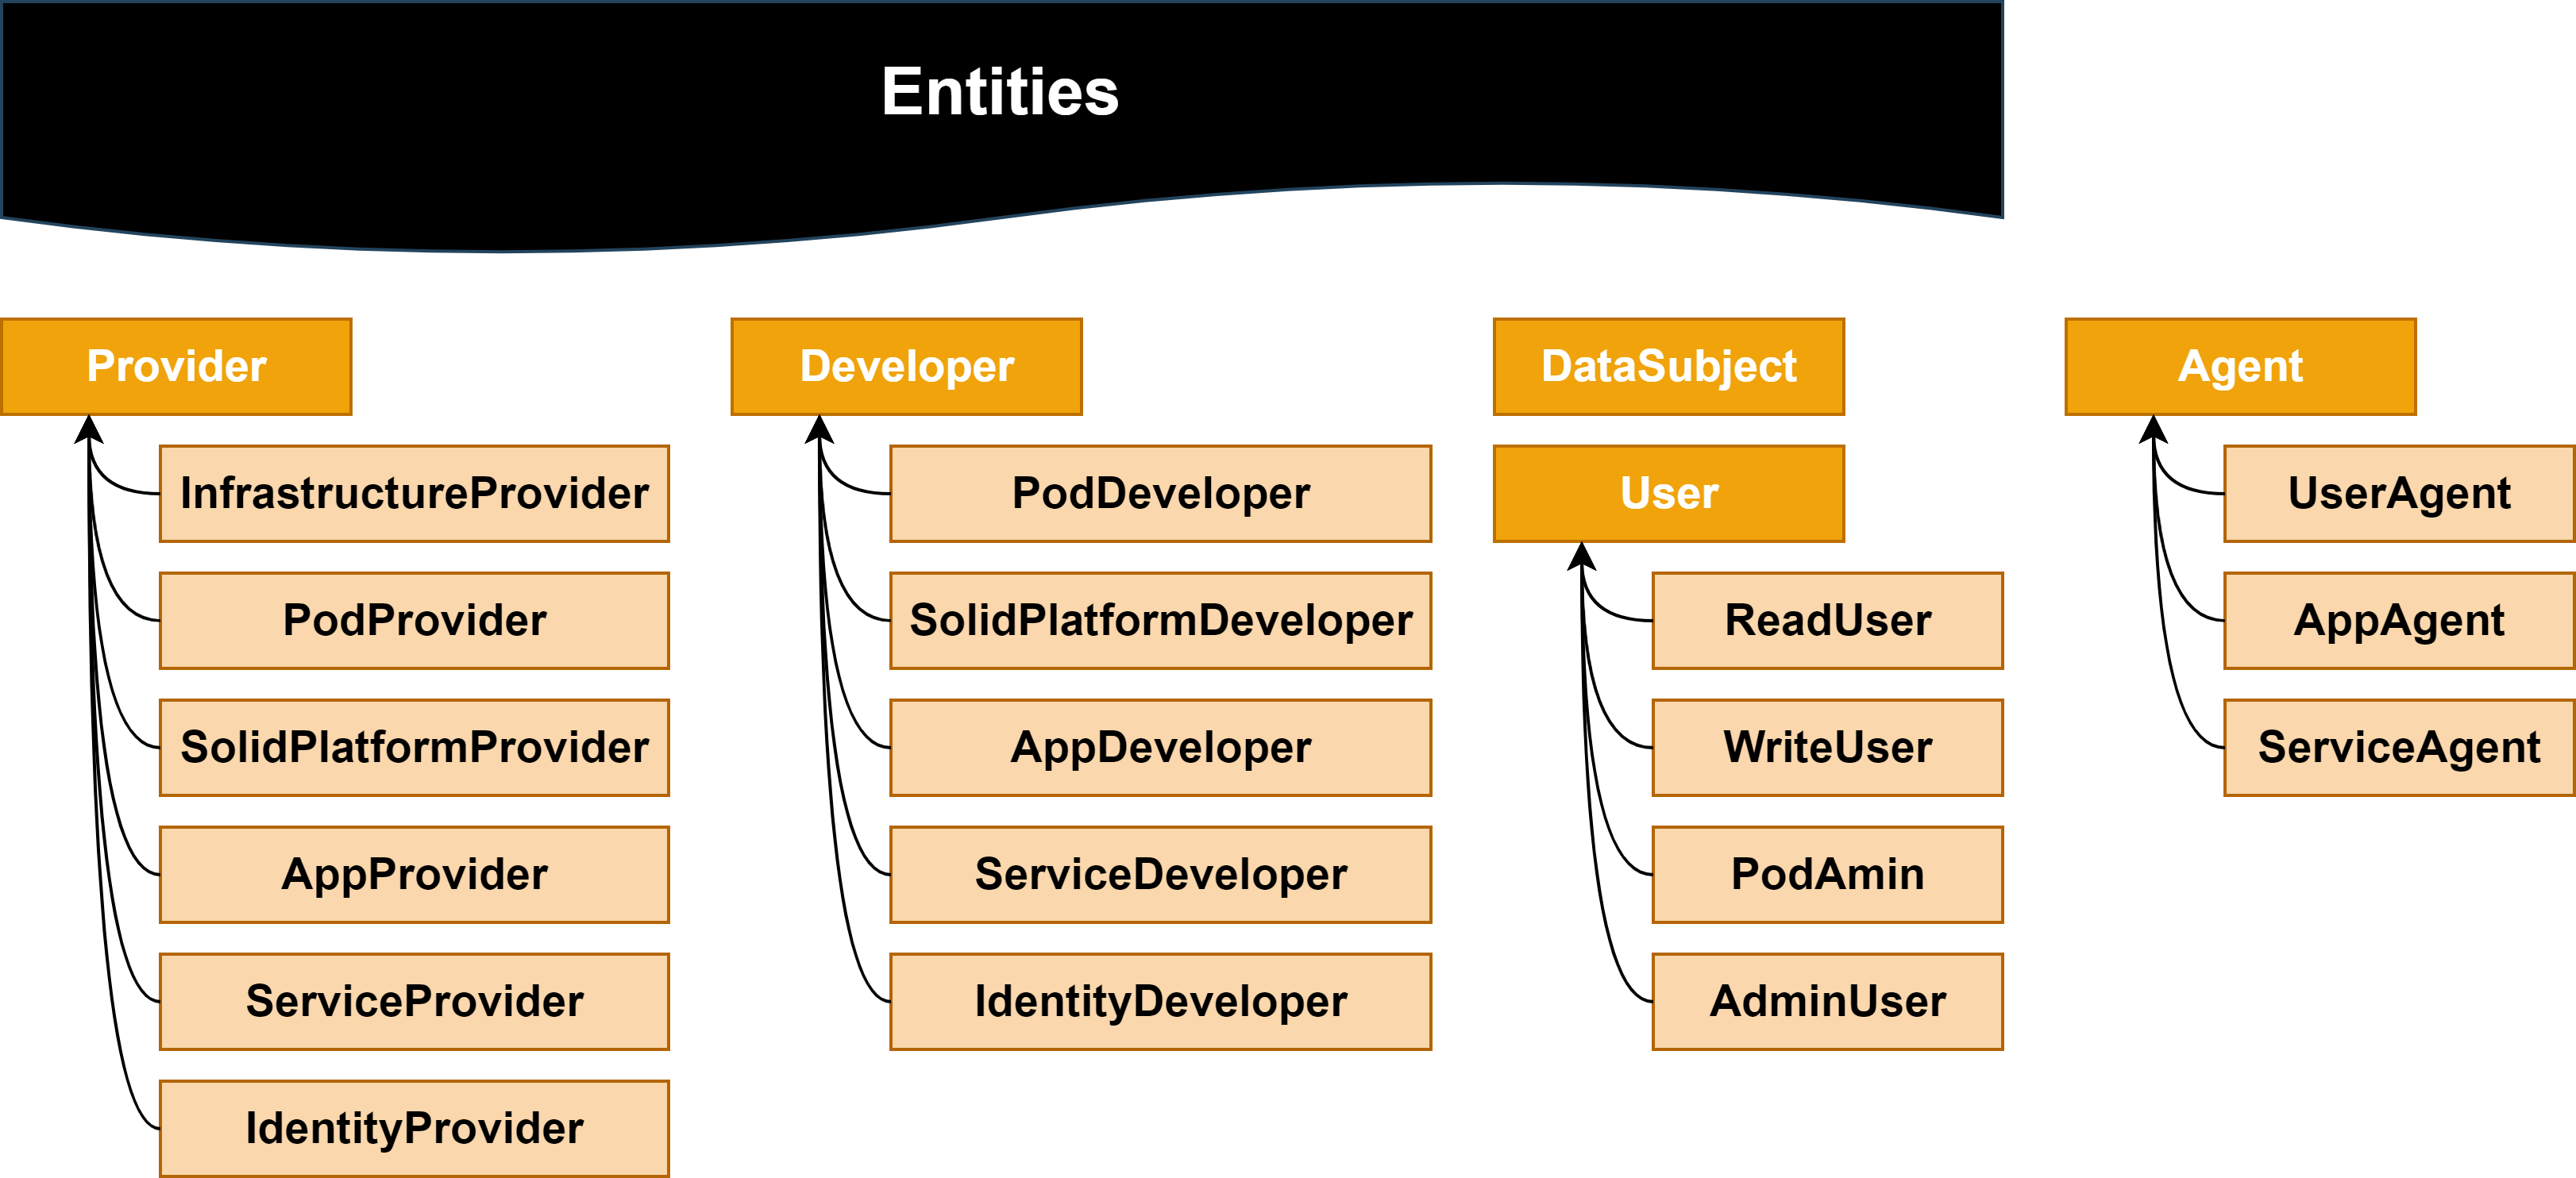
\includegraphics[width=\linewidth]{figures/chapter-4/entities.png}
    \caption{Entities and agents specified in PLASMA.}
    \label{fig:plasma_entities}
\end{figure}

\paragraph{Policies and notices}
In PLASMA, a policy is a document that specifies user, application, and service requirements for data handling practices that apply to data stored or shared through Solid Pods.
Thus, this definition is not limited to access to data stored on a Pod, it also relates to used or transferred data, i.e., to avoid cases such as data collected for purpose X being used for purpose Y.
Such a definition aids with the alignment with legal requirements, e.g., it requires that all purposes must be stated at the time of data collection and that requesters need new consent from the data subject if the purpose for access changes.
PLASMA provides definitions for user policies, in particular for user offers, requirements and preferences, aligned with the \texttt{odrl:Offer}, \texttt{oac:Requirement} and \texttt{oac:Preference} concepts described in Section~\ref{sec:oac}.
Regarding data requests, i.e., conditions for apps and services to have access to or use Pod data, PLASMA envisions their integration into the ecosystem by declaring them in a manifest such as the one being conceived in the W3C Web Application Manifest specification -- an application manifest is a \textit{``JSON document that contains startup parameters and application defaults for when a web application is launched''} \citep{manifest_2023}.
However, the current specification is not enough to achieve legal compliance as it does not include information on entities developing the app, their identity and contact details, or their privacy policies.
Thus, PLASMA includes app manifest and service manifest concepts.
In addition to user policies and data requests, PLASMA also provides different types of data agreements, a concept that is completely missing from the Solid specifications as they only provide concepts to refer to apps and users' access authorisations.
As such, an agreement can either be based on the user's consent, or governed by a contract between the user and the entity having responsibility for the app, service, or Pod.

Additionally, current Solid specifications also lack the definition of notices.
Notices are documents that provide context information about entities, operations, or data involved in specific processes, e.g., notices may specify the providers, developers, and/or data handling practices of applications and services. 
In this regard, PLASMA provides terms for declaring \textit{ex-ante} and \textit{ex-post} notices, i.e., notices declared before and after data access, as well as privacy notices for Pods, users, applications, and services.

Figure~\ref{fig:plasma_policies} illustrates the policies and notices concepts specified in PLASMA.

\begin{figure}[htb]
    \centering
    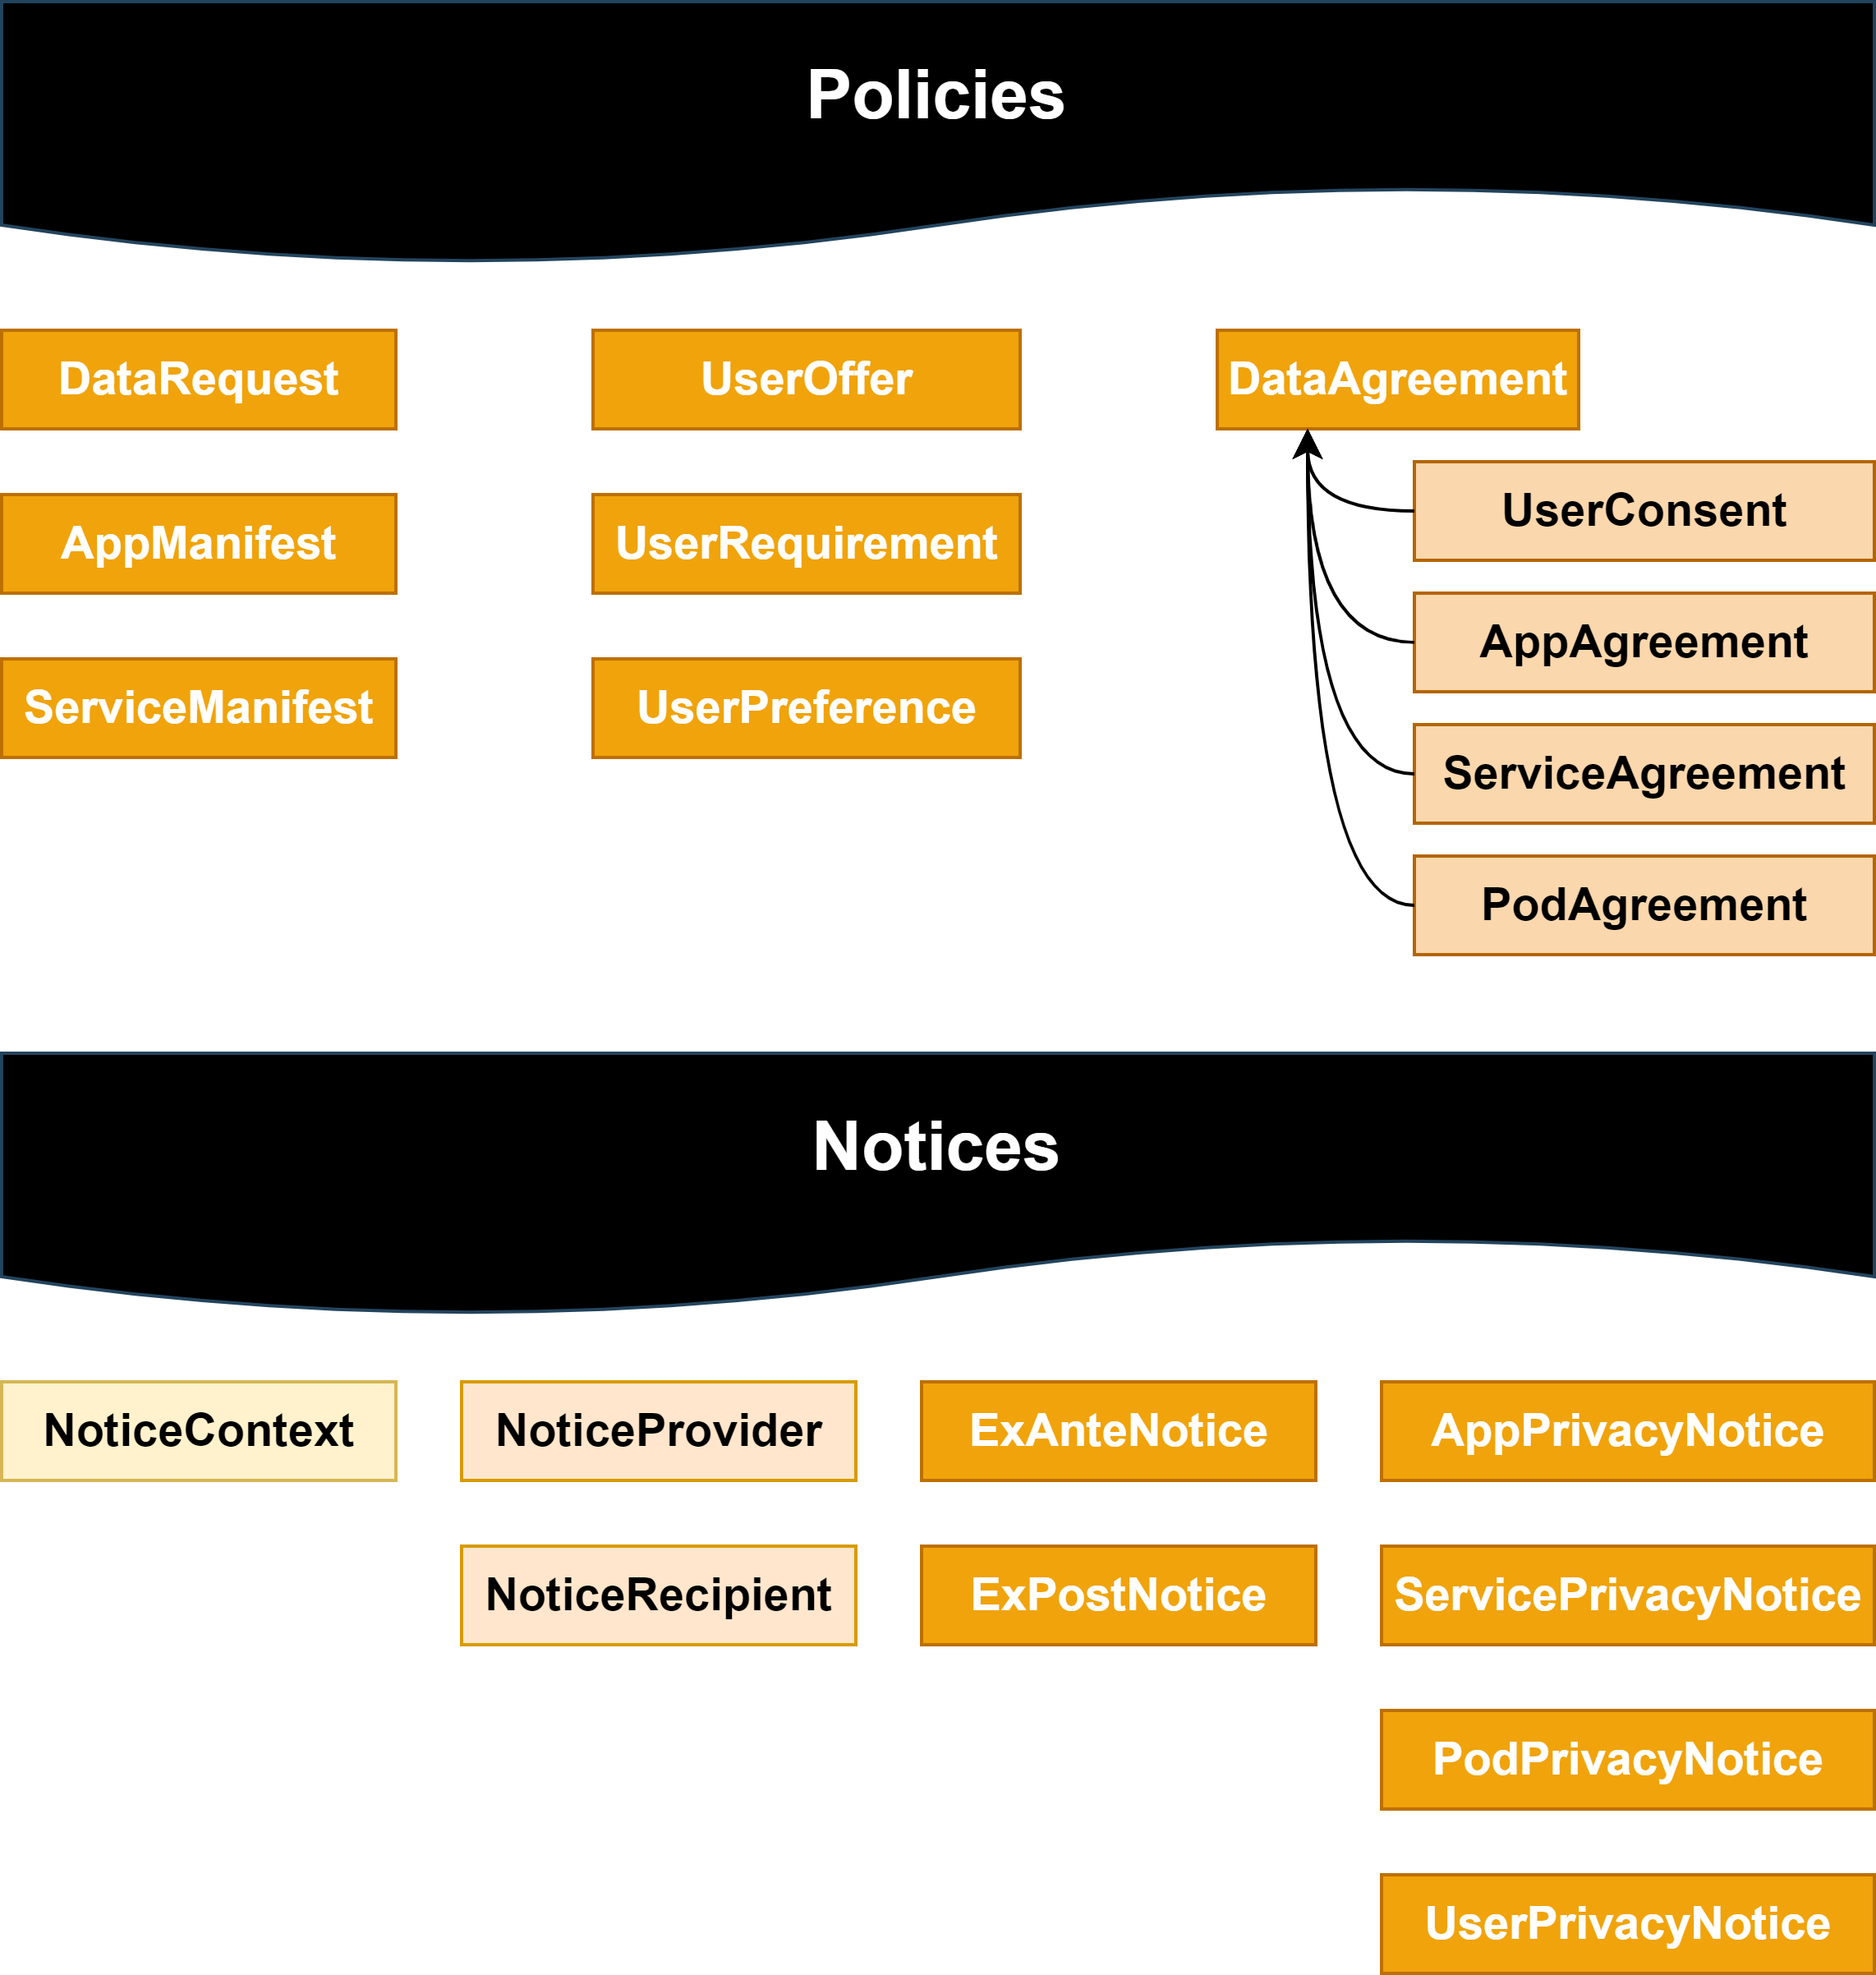
\includegraphics[width=0.8\linewidth]{figures/chapter-4/policies_notices.png}
    \caption{Policy types and notices specified in PLASMA.}
    \label{fig:plasma_policies}
\end{figure}

\paragraph{Services}
PLASMA differentiates between an app and a service -- services convey functionalities that do not need to be packaged as an app.
Moreover, an app requires human intervention to perform some action on data for a specific purpose, while a service may not require human intervention to use or interact with data within a Pod.
Since services are a new concept being introduced by PLASMA in the Solid ecosystem, a taxonomy of twelveu Solid-related services, which can be further expanded, is supplied and illustrated in Figure~\ref{fig:plasma_services}.

\begin{figure}[htb]
    \centering
    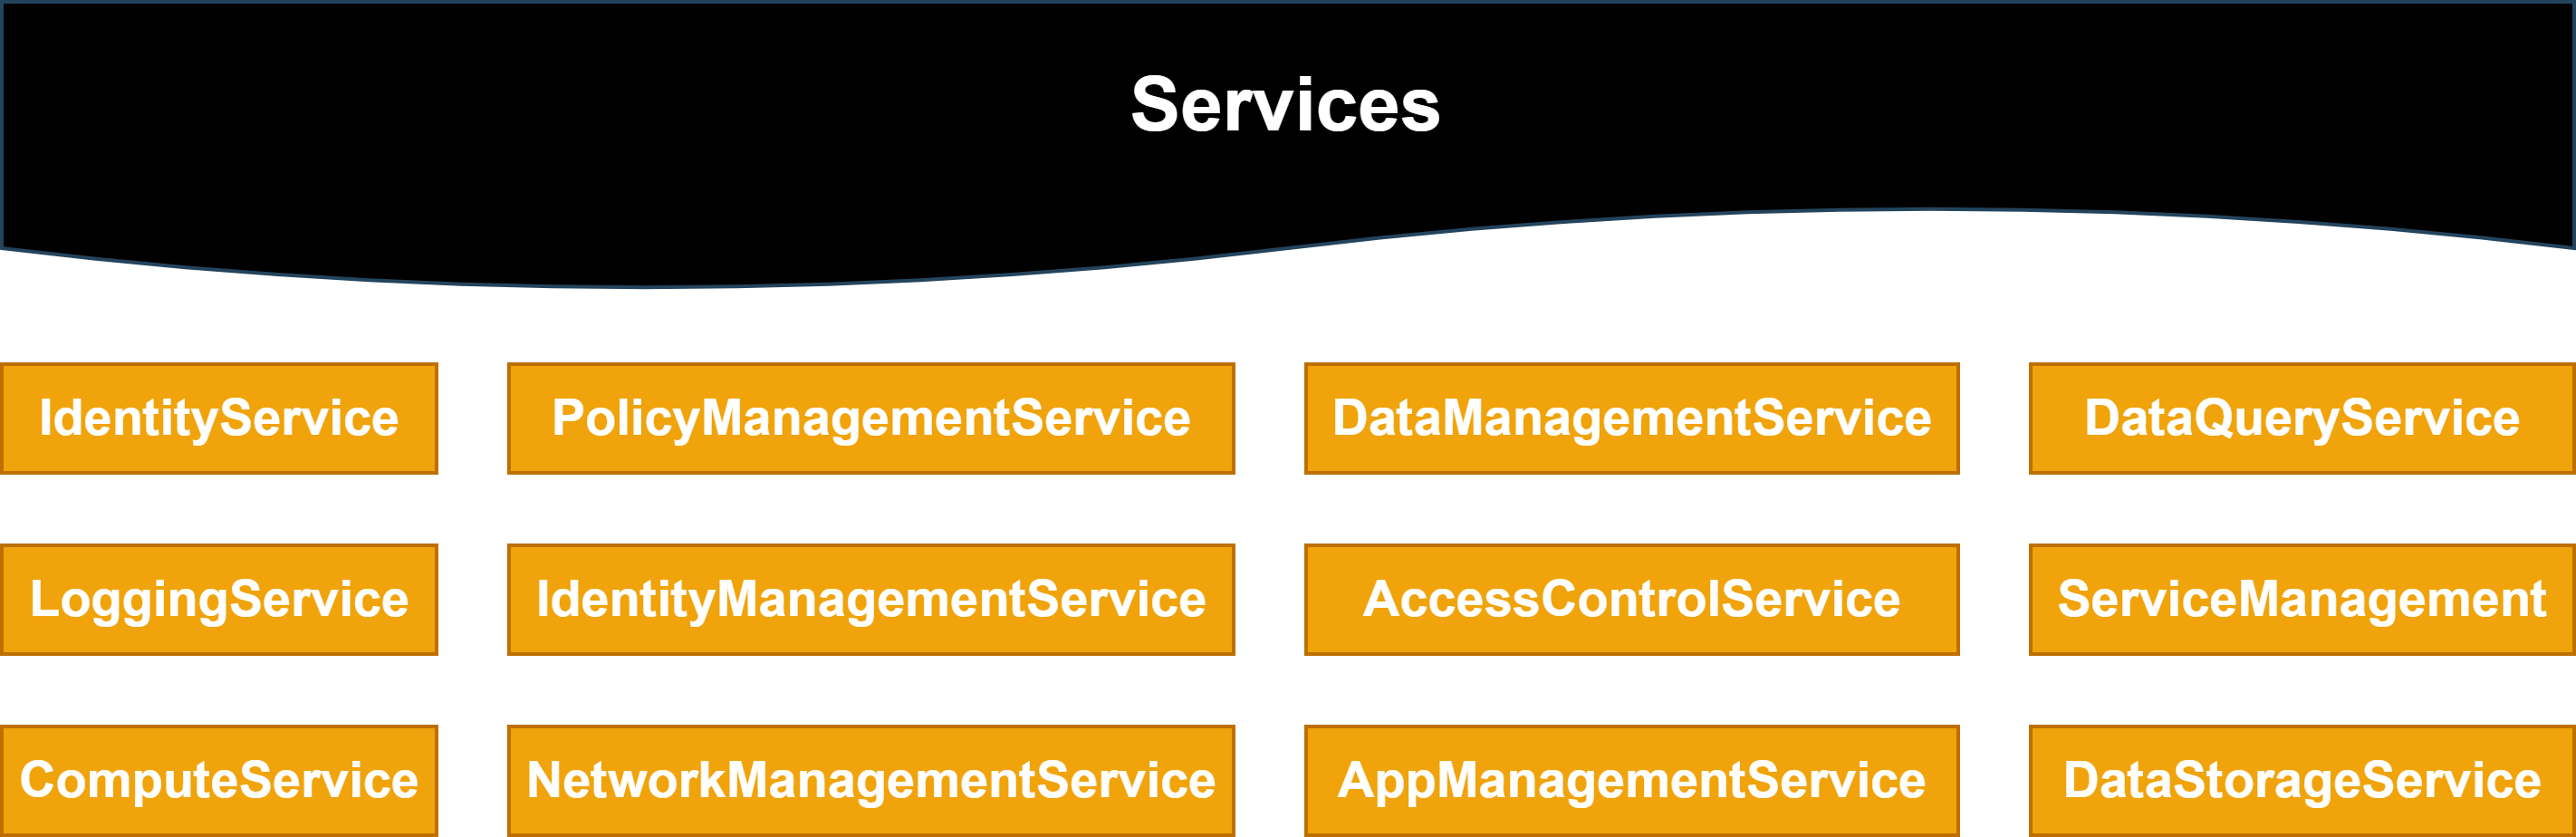
\includegraphics[width=\linewidth]{figures/chapter-4/services.png}
    \caption{Services specified in PLASMA.}
    \label{fig:plasma_services}
\end{figure}

\paragraph{Pod-related data}
To fulfil Solid's vision of providing individuals with a decentralised data storage service for their data and the choice of which applications or services to use for a specific task, metadata regarding Pod management, entities, apps, services, logs and registries should be provided.
Additionally, supervisory authorities can use such logging and provenance metadata, from the Pods of users, for auditing activities, e.g., an EU data protection authority can use these records to investigate a personal data breach.
To this end, PLASMA includes a collection of Solid-related log terms to record provenance information related to processes such as adding or updating resources in a Pod, i.e., a \texttt{DataLog}, registering a policy negotiation procedure reliant on user consent, i.e., a \texttt{PolicyLog}, or recording a successful user login operation, i.e., a \texttt{IdentityLog}.
Furthermore, the maintenance of registries as indexed records for providing collective and convenient access to data within a Pod is of the utmost importance for users, apps, and services to have knowledge of the availability of data categories, supported schemas for data, apps, services, relevant policies, and users that have/had access to data stored within a Pod.

Figure~\ref{fig:plasma_data} illustrates the Pod-related data concepts defined in PLASMA, including logs and registries.

\begin{figure}[htbp]
    \centering
    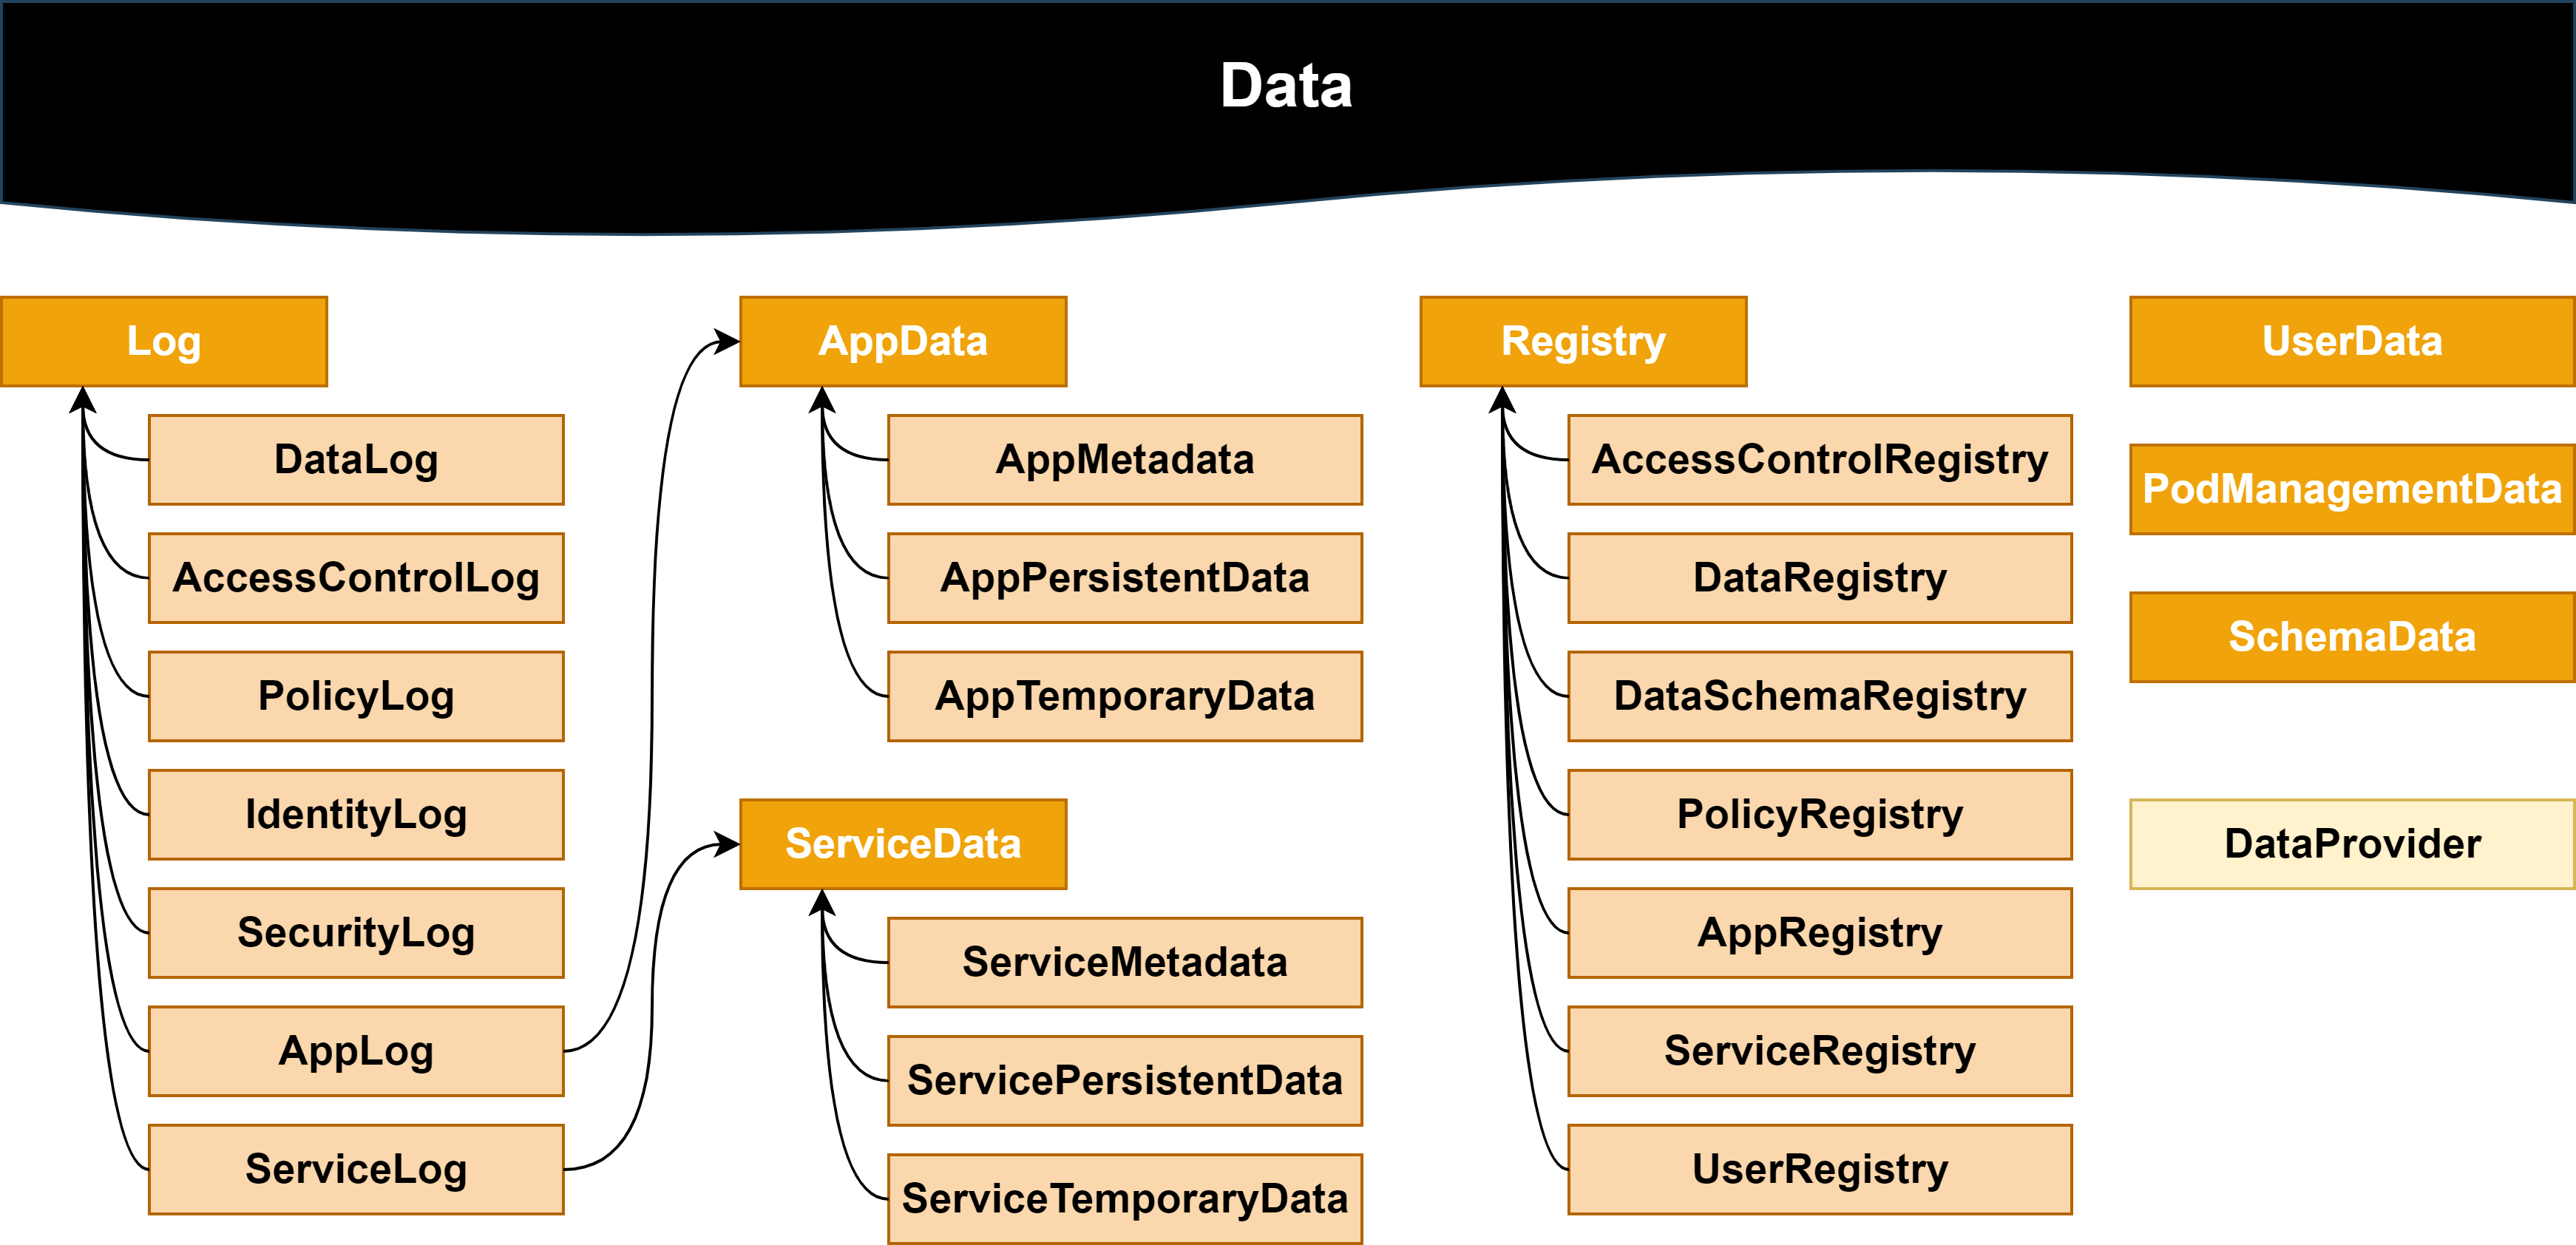
\includegraphics[width=\linewidth]{figures/chapter-4/data.png}
    \caption{Data concepts, including logs and registries, specified in PLASMA.}
    \label{fig:plasma_data}
\end{figure}

\subsection{Conformance with PLASMA}
\label{sec:plasma_conformance}

In this Section, the conditions for Pods, apps, services, users, and agents to be conformant with PLASMA are described, including information regarding what is mandatory (indicated below by the use of the word \textit{must}) or optional (indicated below by the use of the word \textit{may}) to be provided, and how conformity should be evaluated and assured by implementers of the PLASMA specification.
Conformance with these conditions can be checked, e.g., using SHACL shapes.

The W3C Recommendation on Data on the Web Best Practices, which is aimed at the \textit{``publication and usage of data on the Web designed to help support a self-sustaining ecosystem''}~\citep{loscio_data_2017}, was followed for the publication of metadata related to provenance, licensing, and versioning of data.
The vocabulary specifications for particular tasks, recommended by this best practices document, are mentioned in the following paragraphs.
By reusing these concepts, the ontology engineering methodological imperative to maximise the reuse of existing ontological standards to improve interoperability is being followed, as described in the LOT methodology~\citep{poveda-villalon_lot_2022} followed throughout this Thesis.
Table~\ref{tab:reused_vocabs} summarises the reused vocabularies and respective reused terms.
These choices were motivated by the previously mentioned W3C Recommendation on Data on the Web Best Practices, as well as by following ODRL's and DCAT's metadata guidelines, as these are W3C Recommendations for policy expression and dataset, service, and catalog description, respectively.
Their usage is further detailed in each of the conformance sections described below.

\begin{table}[ht]
    \centering
    \caption[Vocabularies reused in PLASMA.]{Vocabularies reused in PLASMA to express conformity of Pods, apps, services, users, and agents.}
    \label{tab:reused_vocabs}
    \begin{tabular}{c||c}
        \textbf{Vocabulary} & \textbf{Reused terms} \\
        \hline\hline
        ODRL & \texttt{hasPolicy} \\
        \hline
        DCMI & \begin{tabular}[c]{@{}c@{}} \texttt{description}, \texttt{source}, \texttt{license}, \texttt{conformsTo}, \texttt{creator},\\ \texttt{created}, \texttt{modified}, \texttt{publisher}, \texttt{format}, \texttt{issued},\\ \texttt{title}, \texttt{language}, \texttt{type}, \texttt{valid} \end{tabular} \\
        \hline
        DPV & \begin{tabular}[c]{@{}c@{}} \texttt{hasName}, \texttt{hasContact}, \texttt{hasAddress},\\ \texttt{hasPolicy}, \texttt{hasNotice}, \texttt{hasDataSubject} \end{tabular} \\
        \hline
        Schema.org & \texttt{codeRepository}\\
        \hline
        PAV & \texttt{version} \\
        \hline
        FOAF & \texttt{page} \\
        \hline
        Activity Streams & \begin{tabular}[c]{@{}c@{}} \texttt{summary}, \texttt{object}, \texttt{actor}, \texttt{generator}, \texttt{Accept},\\ \texttt{Reject}, \texttt{Create}, \texttt{Update}, \texttt{Delete}, \texttt{Move} \end{tabular} \\
    \end{tabular}
\end{table}

% this is a long set of listings that are difficult to follow for reader, could you complement this with a summary onto diagram?

\paragraph{Pod conformance}
For a Pod to be conformant with the PLASMA specification, the following conditions should be satisfied:

\begin{itemize}
    \item A Pod \textit{must} provide or declare \texttt{PodManagementData} which includes metadata about the Pod and of its providers and/or developers, as well as the specific \texttt{SolidPlatform} and \texttt{SolidSpecification} implemented in the Pod and any \texttt{PodAgreement} in place. Listing~\ref{list:plasma_PodManagementData} provides an example of the declaration of such metadata.
    \item A Pod \textit{must} implement or provide equivalent functionality to support the different registries and logs specified in PLASMA. Listing~\ref{list:plasma_dataschemaregistry} provides an example of a data schema registry that records data schemas, formats, or shapes recognised or supported by Pods, apps, or services, as indicated by the \texttt{plasma:supportedBy} property.
    \item A Pod \textit{may} have discovery methods for users to make their data publicly available. These methods \textit{should} rely on the data registries and data schema registries mentioned above.
    \item A Pod \textit{may} have multiple users with varying degrees of control. A record of the different users and their level of access \textit{must} be kept in the \texttt{UserRegistry}.
\end{itemize}

In addition to the ODRL and DCMI Metadata Terms vocabularies, the DPV's \texttt{hasName}, \texttt{hasContact} and \texttt{hasAddress} properties should be used to identify and provide contact details of the Pod, Solid platform and infrastructure providers and developers.
\textit{Schema.org} and the Provenance, Authoring and Versioning (PAV) vocabularies, along with the previously mentioned DCMI, are used to describe the authors, sources, version, and code repository URIs of the platform and specification installed within the Pod.
\textit{Schema.org} provides an upper vocabulary of terms to describe \textit{``entities, relationships between entities and actions''} related to structured data on the Web~\citep{guha_schemaorg_2015} and PAV is a \textit{``lightweight ontology for tracking Provenance, Authoring and Versioning''} that \textit{``specializes the W3C provenance ontology PROV-O in order to describe authorship, curation and digital creation of online resources''}~\citep{ciccarese_pav_2013}.

\begin{listing}[htp]
\caption{Metadata of Beatriz's Pod.}
\label{list:plasma_PodManagementData}
\begin{minted}{turtle}
<https://solidweb.me/besteves4/PodMetadata> a plasma:PodManagementData ;
    dcterms:description "Metadata of Beatriz's Pod" ;
    odrl:hasPolicy <https://solidweb.me/besteves4/agreements/Pod> ;
    plasma:hasProvider <https://solidweb.me/besteves4/entities/PodProvider> ;
    plasma:hasProvider <https://solidweb.me/besteves4/entities/PlatformProvider> ;
    plasma:hasProvider <https://solidweb.me/besteves4/entities/InfrastructureProvider> ;
    plasma:implementedSolidPlatform <https://solidweb.me/besteves4/Platform> ;
    plasma:implementedSolidSpecification <https://solidweb.me/besteves4/SolidSpec> .

<https://solidweb.me/besteves4/agreements/Pod> a plasma:PodAgreement .

<https://solidweb.me/besteves4/entities/PodProvider> a plasma:PodProvider ;
    dpv:hasName "Entity A" ; dpv:hasContact "mailto:entity_a@mail.com" ;
    dpv:hasAddress "Address of Entity A" .

<https://solidweb.me/besteves4/entities/PlatformProvider> a plasma:SolidPlatformProvider .

<https://solidweb.me/besteves4/entities/InfrastructureProvider> a plasma:InfrastructureProvider .

<https://solidweb.me/besteves4/Platform> a plasma:SolidPlatform ;
    plasma:hasProvider <https://solidweb.me/besteves4/entities/PlatformProvider> ;
    dcterms:source <https://communitysolidserver.github.io> ;
    dpv:hasPolicy <https://www.serverproject.de/files/solidweb_me_terms.txt> ;
    schema:codeRepository <https://github.com/CommunitySolidServer/CommunitySolidServer> ;
    pav:version "6.1.0" ;
    dcterms:license <https://dalicc.net/licenselibrary/MIT> .

<https://solidweb.me/besteves4/SolidSpec> a plasma:SolidSpecification ;
    dcterms:conformsTo <https://solidproject.org/TR/2022/protocol-20221231> ;
    dcterms:creator "Sarven Capadisli", "Tim Berners-Lee", "Ruben Verborgh", "Kjetil Kjernsmo" ;
    dcterms:license <https://dalicc.net/licenselibrary/MIT> ;
    pav:version "0.10.0" ; dcterms:created "2022-12-31"^^xsd:date ;
    schema:codeRepository <https://github.com/solid/specification> .
\end{minted}
\end{listing}

\begin{listing}[htp]
\caption{Data schema registry of Beatriz's Pod.}
\label{list:plasma_dataschemaregistry}
\begin{minted}{turtle}
<https://solidweb.me/besteves4/SchemaRegistry> a plasma:DataSchemaRegistry ;
    dcterms:description "Registry listing recognised or supported schemas" ;
    dcterms:created "2023-09-10T11:51:17"^^xsd:dateTime ;
    dcterms:modified "2023-10-07T12:39:50"^^xsd:dateTime ;
    dcterms:publisher <https://solidweb.me/besteves4/entities/DataMgtServiceProvider> ;
    plasma:hasSchema <https://solidweb.me/besteves4/schemas/EHR-schema>,
        <https://solidweb.me/besteves4/schemas/img-format>,
        <https://solidweb.me/besteves4/schemas/entity-shape> .

<https://solidweb.me/besteves4/entities/DataMgtServiceProvider> a plasma:ServiceProvider ;
    plasma:serviceType plasma:DataManagementService ;
    dpv:hasName "Entity A" ;
    dpv:hasAddress "Address of Entity A" ;
    dpv:hasContact "mailto:entity_a@mail.com" .

<https://solidweb.me/besteves4/schemas/EHR-schema> a plasma:SchemaData ;
    dcterms:conformsTo <http://www.w3.org/TR/turtle/> ;
    plasma:supportedBy <https://example.com/health-service> .

<https://example.com/health-service> a plasma:Service .

<https://solidweb.me/besteves4/schemas/img-format> a plasma:SchemaData ;
    dcterms:format <https://www.iana.org/assignments/media-types/image/png>,
        <https://www.iana.org/assignments/media-types/image/svg+xml> ;
    plasma:supportedBy <https://example.com/social-app> .

<https://example.com/social-app> a plasma:App .

<https://solidweb.me/besteves4/schemas/entity-shape> a plasma:SchemaData, sh:NodeShape ;
    plasma:supportedBy <https://solidweb.me/besteves4/> ;
    sh:name "PLASMA entity shape" ;
    sh:description "Minimum data that PLASMA entities should provide to be identified." ;
    sh:targetClass plasma:Entity .
\end{minted}
\end{listing}

\paragraph{Apps and services conformance}
For an app or service to be conformant with the PLASMA specification, the following conditions should be satisfied:

\begin{itemize}
    \item An app, or service, \textit{must} have an \texttt{AppManifest}, or \texttt{ServiceManifest}, in conformance with the W3C Web Application Manifest \citep{manifest_2023}. Listing~\ref{list:plasma_appmanifest} provides an example of such an app manifest.
    \item An \texttt{AppManifest}, or \texttt{ServiceManifest}, \textit{must} include information regarding the developer and provider of legally relevant entities and their identities.
    \item An \texttt{AppManifest}, or \texttt{ServiceManifest}, \textit{must} state the \texttt{DataRequest} representing the request to use data using the \texttt{odrl:hasPolicy} property. The request \textit{must} provide all information regarding the use of data even if only some of it will be applicable initially or used in the notice.
    \item An \texttt{AppManifest}, or \texttt{ServiceManifest}, \textit{must} link the privacy notice of the app, or service, using the \texttt{dpv:hasNotice} property. The Pod \textit{may} use this information to display or optionally construct its own notice based on the preferences or accessibility requirements of the user.
    \item An \texttt{AppManifest}, or \texttt{ServiceManifest}, \textit{must} be stored in the Pod \texttt{AppRegistry}, or \texttt{ServiceRegistry}. Listing~\ref{list:plasma_appregistry} provides an example of an app registry, where app-related metadata, including the manifest, app providers and developers, temporary or persistent app data, is recorded.
    \item Apps, or services, \textit{may} have multiple \texttt{AppAgents}, or \texttt{ServiceAgents}, which \textit{must} be registered in the \texttt{AppRegistry}, or \texttt{ServiceRegistry}.
\end{itemize}

In addition to the PLASMA terms mentioned in the previous list, the usage of the \texttt{plasma:serviceType} property can be used to connect service providers and developers with a particular type of service, e.g., from PLASMA's service taxonomy, that is provided or developed by said entity.
Moreover, it should be noted that app or service stores, such as those maintained by Apple and Google, can also act as app or service providers and the FOAF \texttt{page} property can be used to actually connect the store provider with the store itself.
The FOAF vocabulary specification~\citep{brickley_foaf_2004} provides terms to describe people and related personal information and online accounts.
Regardless, support for other optional properties specified in the W3C Web Application Manifest specification, such as icons, display mode, orientation, and background colour, can also be integrated into the modelled manifests, as well as `common' app store metadata, such as screenshots, user rating or app type, e.g., health, game or news app~\citep{gustafson_web_2023}.

\begin{listing}[htp]
\caption{App manifest of Contacts app.}
\label{list:plasma_appmanifest}
\begin{minted}{turtle}
<https://example.com/Contacts> a plasma:App ;
    plasma:hasAppManifest <https://example.com/Contacts/Manifest> .

<https://example.com/Contacts/Manifest> a plasma:AppManifest ;
    dcterms:conformsTo <https://www.w3.org/TR/appmanifest/> ;
    dcterms:issued "2023-10-23T22:43:58"^^xsd:dateTime ;
    dcterms:title "Contacts" ;
    dcterms:description "App to manage contacts" ;
    dcterms:language <http://id.loc.gov/vocabulary/iso639-1/en> ;
    plasma:hasProvider <https://solidweb.me/besteves4/entities/AppStore> ;
    plasma:hasDeveloper <https://solidweb.me/besteves4/entities/ContactsDeveloper> ;
    odrl:hasPolicy <https://example.com/Contacts/Request> ;
    dpv:hasNotice <https://example.com/Contacts/Notice> .

<https://solidweb.me/besteves4/entities/AppStore> a plasma:AppProvider ;
    dpv:hasName "App Store provider" ;
    dpv:hasAddress "Address of App Store provider" ;
    dpv:hasContact "mailto:app_store@mail.com" ;
    foaf:page <https://example.com/AppStore> ;
    dpv:hasNotice <https://example.com/AppStore/PrivacyPolicy> .

<https://solidweb.me/besteves4/entities/ContactsDeveloper> a plasma:AppDeveloper .

<https://example.com/Contacts/request> a plasma:DataRequest, odrl:Request .
\end{minted}
\end{listing}

\begin{listing}[htp]
\caption{App registry of Beatriz's Pod.}
\label{list:plasma_appregistry}
\begin{minted}{turtle}
<https://solidweb.me/besteves4/AppRegistry> a plasma:AppRegistry ;
    dcterms:description "Registry listing apps" ;
    dcterms:created "2023-09-30T11:33:35"^^xsd:dateTime ;
    dcterms:modified "2023-10-07T11:31:40"^^xsd:dateTime ;
    dcterms:publisher <https://solidweb.me/besteves4/entities/AppMgProvider> ;
    plasma:hasApp <https://solidweb.me/besteves4/apps/Contacts/> .

<https://solidweb.me/besteves4/entities/AppMgProvider> a plasma:ServiceProvider ;
    plasma:serviceType plasma:AppManagementService .

<https://solidweb.me/besteves4/apps/Contacts/> a plasma:App ;
    plasma:hasAppManifest <https://solidweb.me/besteves4/apps/Contacts/Manifest> ;
    odrl:hasPolicy <https://solidweb.me/besteves4/apps/Contacts/Agreement> ;
    plasma:hasAppMetadata <https://solidweb.me/besteves4/apps/Contacts/Metadata> ;
    plasma:hasAppPersistentData <https://solidweb.me/besteves4/apps/Contacts/PersistentData> ;
    plasma:hasAppTemporaryData <https://solidweb.me/besteves4/apps/Contacts/TemporaryData> ;
    plasma:hasAgent <https://solidweb.me/besteves4/apps/Contacts/Agent> .

<https://solidweb.me/besteves4/apps/Contacts/Metadata> a plasma:AppMetadata ;
    dcterms:description "Contacts metadata" ;
    plasma:hasProvider <https://solidweb.me/besteves4/entities/AppStore> ;
    plasma:hasDeveloper <https://solidweb.me/besteves4/entities/ContactsDeveloper> .

<https://solidweb.me/besteves4/apps/Contacts/PersistentData> a plasma:AppPersistentData ;
    dcterms:type dpv-pd:TelephoneNumber ; rdf:value "(+34)691485135" .

<https://solidweb.me/besteves4/apps/Contacts/TemporaryData> a plasma:AppTemporaryData ;
    dcterms:type dpv-pd:TelephoneNumber ; rdf:value "(+34)691998745" ;
    dcterms:valid "2023-10-01T14:50:21"^^xsd:dateTime .

<https://solidweb.me/besteves4/apps/Contacts/Agent> a plasma:AppAgent .
\end{minted}
\end{listing}

\paragraph{User conformance}
For a user to be conformant with the PLASMA specification, the following conditions should be satisfied:

\begin{itemize}
    \item Impactful interactions of a user, e.g., changing identity providers, \textit{must} be recorded using a well-defined shape. Listing~\ref{list:plasma_accesscontrollog} provides an example of access control logs modelled with PLASMA and using W3C's Activity Streams activity types~\citep{snell_activity_2017}.
    \item A \texttt{UserRegistry} \textit{must} contain information regarding the \texttt{DataSubjects} storing data within a Pod, the \texttt{PodAdmin} and other users accessing Data. Listing~\ref{list:plasma_userregistry} provides an example of said registry.
    \item Users \textit{may} be directly associated with a \texttt{DataRequest} so that they can make requests for data without using an application or service.
    \item Users \textit{may} have multiple \texttt{UserAgents}, which should be registered in the \texttt{UserRegistry}.
\end{itemize}

PLASMA recommends the usage of the W3C's Activity Streams vocabulary~\citep{snell_activity_2017} to model the distinct logs that should be stored in Solid Pods for transparency and accountability, e.g., data, identity, or policy logs.
This recommendation provides an extensive list of activity, actor, and object types that provides \textit{``a baseline extensible syntax for the expression of completed activities''}.
Such syntax allows the identification of the resource being logged, using the \texttt{as:object} property, the entity responsible for the activity being logged, using the \texttt{as:actor} property, or the app or service used to generate the log, employing the \texttt{as:generator} property.
The \texttt{as:Accept} and \texttt{as:Reject} activity types can be reused to express when access to data or policies is accepted or rejected, and the \texttt{as:Create}, \texttt{as:Update}, \texttt{as:Delete} and \texttt{as:Move} activities can be reused to log the creation, modification, deletion or movement of data or policies.
New activity types, e.g., to request data, change identity providers, or verify the identity of apps, which are not modelled by the Activity Streams vocabulary, are modelled in PLASMA, e.g., as \texttt{plasma:Request}, \texttt{plasma:ChangeIdP} or \texttt{plasma:Verify}.

It should also be stated that Inrupt's Enterprise Solid Server has started to provide an auditing service\footnote{\url{https://docs.inrupt.com/ess/latest/services/service-auditing/} (accessed on 21 December 2023)} which also relies on the W3C Activity Streams 2.0 Recommendation~\citep{snell_activity_2017} to document audit events related with the identity of user and applications.

\begin{listing}[htp]
\caption{Access control logs recorded in Beatriz's Pod.}
\label{list:plasma_accesscontrollog}
\begin{minted}{turtle}
<https://solidweb.me/besteves4/logs/AccessControl_Reject> a plasma:AccessControlLog ;
	dcterms:type as:Reject ;
	dcterms:issued "2023-11-12T15:34:04"^^xsd:dateTime ;
	as:summary "Access to data rejected" ;
	as:object <https://solidweb.me/besteves4/health/ehr> ;
	as:actor <https://solidweb.me/arya/profile/card#me> ;
	as:generator <https://example.com/App> ;
	dcterms:publisher <https://solidweb.me/besteves4/entities/LoggingProvider> .

<https://solidweb.me/besteves4/logs/AccessControl_Accept> a plasma:AccessControlLog ;
	dcterms:type as:Accept ;
	dcterms:issued "2023-11-12T15:43:09"^^xsd:dateTime ;
	as:summary "Access to data accepted" ;
	as:object <https://solidweb.me/besteves4/contacts/> ;
	as:actor <https://solidweb.me/arya/profile/card#me> ;
	as:generator <https://example.com/App> ;
	dcterms:publisher <https://solidweb.me/besteves4/entities/LoggingProvider> .

<https://example.com/App> a plasma:App .

<https://solidweb.me/besteves4/entities/LoggingProvider> a plasma:ServiceProvider ;
	plasma:serviceType plasma:LoggingService ;
	dpv:hasName "Entity G" ;
	dpv:hasAddress "Address of Entity G" ;
	dpv:hasContact "mailto:entity_g@mail.com" .
\end{minted}
\end{listing}

\begin{listing}[htp]
\caption{User registry of Beatriz's Pod.}
\label{list:plasma_userregistry}
\begin{minted}{turtle}
<https://solidweb.me/besteves4/UserRegistry> a plasma:UserRegistry ;
    dcterms:description "Registry listing users" ;
    dcterms:created "2023-09-30T11:33:35"^^xsd:dateTime ;
    dcterms:modified "2023-10-07T12:39:50"^^xsd:dateTime ;
    dcterms:publisher <https://solidweb.me/besteves4/entities/UserMProvider> ;
    dpv:hasDataSubject <https://solidweb.me/besteves4/entities/DataSubject> ;
    plasma:hasUser <https://solidweb.me/besteves4/entities/DataSubject>,
        <https://solidweb.me/besteves4/entities/ReadUserA>,
        <https://solidweb.me/besteves4/entities/ReadUserB>,
        <https://solidweb.me/besteves4/entities/Admin> .

<https://solidweb.me/besteves4/entities/UserMProvider> a plasma:ServiceProvider ;
    dpv:hasName "Entity A" ;
    dpv:hasAddress "Address of Entity A" ;
    dpv:hasContact "mailto:entity_a@mail.com" .

<https://solidweb.me/besteves4/entities/DataSubject> a plasma:DataSubject, plasma:PodAdmin ;
    dpv:hasName "Data Subject" ;
    dpv:hasAddress "Address of Data Subject" ;
    dpv:hasContact "mailto:data_subject@mail.com" ;
    plasma:hasAgent <https://solidweb.me/besteves4/agents/AgentA> .

<https://solidweb.me/besteves4/agents/AgentA> a plasma:UserAgent .

<https://solidweb.me/besteves4/entities/ReadUserA> a plasma:ReadUser ;
    plasma:hasPolicy <https://solidweb.me/besteves4/requests/UserA> .

<https://solidweb.me/besteves4/entities/UserA> a plasma:DataRequest .

<https://solidweb.me/besteves4/entities/ReadUserB> a plasma:ReadUser ;
    plasma:hasPolicy <https://solidweb.me/besteves4/requests/UserB> ;
    plasma:hasPolicy <https://solidweb.me/besteves4/agreements/UserB> .

<https://solidweb.me/besteves4/agreements/UserB> a odrl:Agreement, plasma:UserConsent .

<https://solidweb.me/besteves4/entities/Admin> a plasma:AdminUser .
\end{minted}
\end{listing}

\paragraph{Agent conformance}
For an agent to be conformant with the PLASMA specification, the following conditions should be satisfied:

\begin{itemize}
    \item Agents activity \textit{must} be in accordance with the manifest of the entity for which they are acting on behalf of. As such, agents \textit{must} follow the policies of the entities they are acting on behalf of.
    \item A record of the usage of an \texttt{AppAgent}, \texttt{ServiceAgent} or \texttt{UserAgent} \textit{must} be kept in the \texttt{AppRegistry}, \texttt{ServiceRegistry} or \texttt{UserRegistry}, respectively, including information regarding its providers/developers for accountability. User \url{https://solidweb.me/besteves4/entities/DataSubject} in Listing~\ref{list:plasma_userregistry} has a user agent identified with the PLASMA property \texttt{hasAgent}.
\end{itemize}

Finally, each of the requirements established in the previous paragraphs for the conformance of Pods, apps, services, users, and agents with PLASMA should be verified using a language for describing and validating RDF graphs.
As such, SHACL can, not only, be used for the definition of data shapes recognised or supported by apps, services, or Pods, but also can act as a general tool to verify conformance with the conditions specified in this Section.
SHACL was chosen for this conformance checking since it is a widely used and supported W3C Recommendation for \textit{``validating RDF graphs against a set of conditions''}~\citep{knublauch_shapes_2017}.
As such, a SHACL validation tool takes a data graph and a shapes graph as input and produces a validation report that contains the outcomes of the validation.
This validation report includes a set of all validation results, one for each shape being evaluated, which can be positive or negative, according to the result of the validation. 
SHACL shapes for all the previously mentioned conformance conditions were generated in this Thesis, and are available in PLASMA's online documentation and source code repository.
Hence, conformance with the PLASMA specification relies on the proper modelling of policies, logs, registries and other metadata, using the terms suggested by the specification, i.e., for actual interoperability between Pods, apps, services, users, and agents.
Moreover, SHACL validation reports can be used to assess which conformance conditions are not being met.
While such reports are not enough to identify malicious actors, they can be used to advice users against using Pod, app, service, or agent providers which do not adhere to PLASMA's conformance conditions, and to ensure that the necessary metadata is available to the user in case such malicious uses are found, e.g., to be used by the data subject to lodge a complaint.

% it would be good to include a table mapping the earlier conformance statements against specific shaql shapes to help convey this coverage.

% SHACL shapes generator: https://github.com/AKSW/shaclgen

\subsection{Vocabulary publication and maintenance}
\label{sec:plasma_publication}

The vocabulary human-readable documentation and machine-readable file are available at \url{https://w3id.org/plasma} using content negotiation.
The HTML documentation includes a description of the terms defined in PLASMA, which was conducted and validated with domain experts\footnote{This validation was performed with experts on the Solid technology, namely during the Short-Term Scientific Mission at the \textit{KNoWS} group, as well as with the contacts made at \textit{Inrupt}.}, diagrams with graphical representations of the several taxonomies included in the vocabulary, a detailed explanation of the conformance conditions that need to be adopted by Pods, apps, services, agents and users for them to be PLASMA-compliant, RDF examples of workflows that use PLASMA terms for specific scenarios, e.g., creating user policies or auditing Pods, and information related to legal compliance.
The vocabulary documentation also includes metadata, such as the identity of the creators and publishers of the ontology, the dates of creation and last modification, or the version number.

The source code is hosted at \url{https://w3id.org/plasma/repo}, under the CC-BY-4.0 license.
The repository can also be used by PLASMA implementers to suggest new inclusions to the vocabulary and to report bugs through GitHub Issues.